\newpage
\section{Training neural network models with single hidden layer}

So far we've only trained our model through a simple perceptron which includes one input layer and one output layer. The output layer was a single node which received its input from the previous layer, and this input was a weighted sum of the weights at each of the input nodes multiplied by the input values. This weighted sum was passed to a sigmoid activation function. We then computed the loss and updated the weights through back propagation.

In this chapter, we will create a neural network model with one input layer, one hidden layer and one output layer. The architecture of the neural network model will look as below:

\begin{figure}[htbp]
\centering
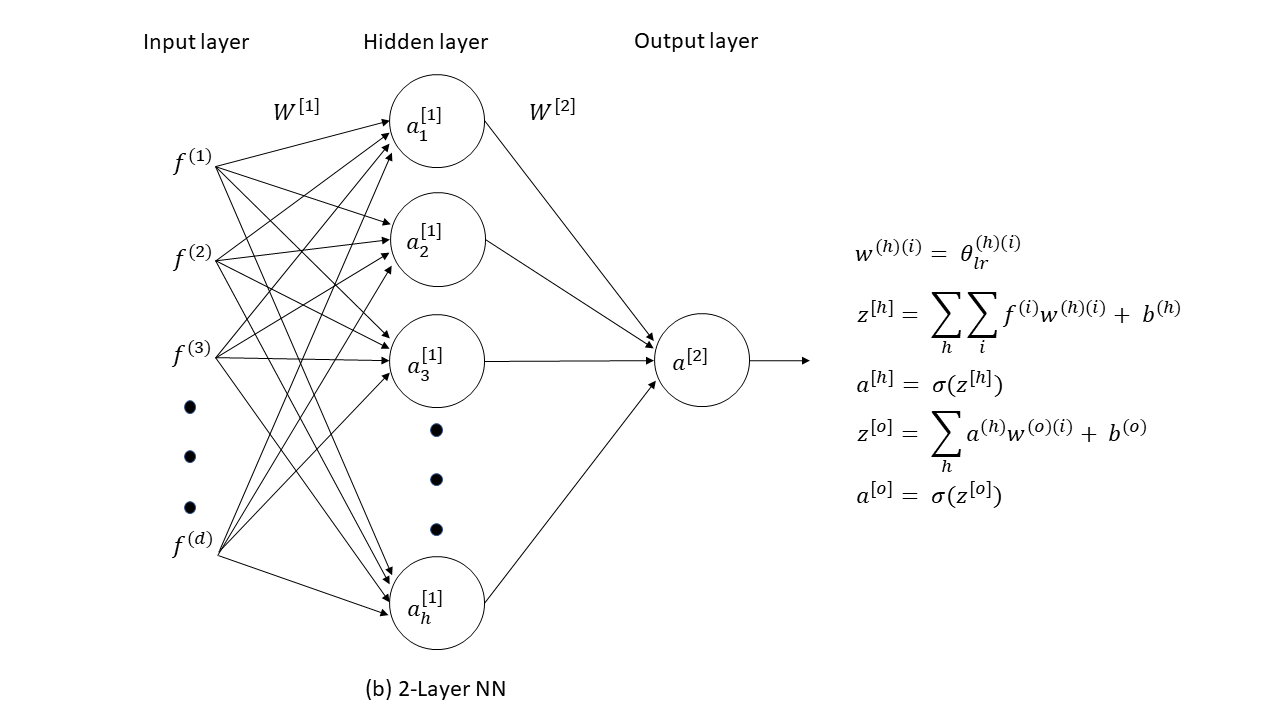
\includegraphics[width=16cm, height=10cm]{images/nn1.png}\\
\centering
\caption{Neural network model - without using word-vectors}
\label{fig:foo}
\end{figure}

In the figure above, we have a neural network with one input layer having d features, one hidden layer and one output layer. For the case of simplicity we assume we are trying to solve a binary classification problem, where there can be only two possible outputs. In reality, for multi-class classification problems, the output layer will contain multiple nodes equivalent to the total number of classes. This neural network is also capable of finding non-linear boundaries.

No matter how many nodes and hidden layers are there in a neural network, the basic working principle remains the same. We compute what the hypothesis outputs given an input through the forward propagation stage and through back propagation find the best weights that minimize the cost function.

We will build two separate models, one that uses the word-vector weights in the input layer and the one that doesn't. We then compare both model performances to see whether using the word-vector weights has improved the model performance or not.

\subsection{Neural Network model without word-vectors}

The neural network model without word-vectors is similar to using a logistic regression model with one extra hidden layer. We can look at how to perform feed-forward and back-propagation steps for this neural network.\\

\noindent \textbf{Feed Forward:}\\

We know that the input for node $j$ in layer $l$ is the weighted sum of the activation outputs from the previous layer $l-1$. So, the input for a given hidden node $h$ is expressed as:

\begin{equation}
z^{[h]} = \sum_{h}\sum_{i} f^{(i)}w^{(h)(i)} + b^{(h)}
\end{equation}

where, $f^{(i)}$ is the feature value of feature $i$

$\quad\qquad\ w^{(h)(i)} = \theta_{lr}^{(h)(i)}$ is the weight of hidden layer $h$ for input feature $i$

$\quad\qquad\ b$ is the bias added to the network\\

To that input node, we apply the activation function which in our case would be a sigmoid activation function given as:

\begin{equation}
a^{[h]} = \sigma(z^{[h]})
\end{equation}

where, $\sigma$ is the sigmoid activation function given as $\frac{1}{1+e^{-z^[h]}}$\\

This activation function output for each hidden layer is then passed as part of the input for the node in the output layer to which a sigmoid function is applied for binary classification.

\begin{equation}
z^{[o]} = \sum_{h} a^{(h)}w^{(o)(i)} + b^{(o)}
\end{equation}

\begin{equation}
a^{[o]} = \sigma(z^{[o]})
\end{equation}

\noindent \textbf{Back Propagation:}\\

Once we reach the output layer, we obtain the resulting output from the model for the given input. We then compute the loss which is the difference between the predicted and actual output.

\begin{equation}
\frac{\partial cost}{\partial a^{[o]}} = a^{[o]}-y
\end{equation}

Our objective is to minimize the loss by updating the weights of the output layer and the hidden layer. The loss of an individual node is actually a function of the activation output for that node, which itself is a function of the input to that node, and that input is a function of the weights that connect all the nodes in the previous layer to this node. Thus, the loss function is actually a composition of all of these functions.

To differentiate a composition of functions, we use the chain rule. We're needing to calculate derivatives that depend on components later in the network first and then use these derivatives in our calculations for the gradient of the loss wrt the weights that come earlier in the network. So we achieve this by repeatedly applying the chain rule in the backwards fashion.\\

\noindent Using the chain rule, the change in cost wrt weights $w^{[o]}$ and $w^{[h]}$ is given as:

\begin{equation}
\frac{\partial cost}{\partial w^{[o]}} = \frac{\partial cost}{\partial a^{[o]}} * \frac{\partial a^{[o]}}{\partial z^{[o]}} * \frac{\partial z^{[o]}}{\partial w^{[o]}}
\end{equation}

\begin{equation}
\frac{\partial cost}{\partial w^{[h]}} = \frac{\partial cost}{\partial a^{[h]}} * \frac{\partial a^{[h]}}{\partial z^{[h]}} * \frac{\partial z^{[h]}}{\partial w^{[h]}}
\end{equation}

where, $\frac{\partial a^{[o]}}{\partial z^{[o]}} =  \sigma^{'}(z^{[o]})$\\

$\quad\qquad\ \frac{\partial z^{[h]}}{\partial w^{[h]}} = a^{[h]}$ \\

The partial derivatives of the hidden layer can also be computed in a similar way. We can then update the weights as:

\begin{equation}
w^{[o]} = w^{[o]} - lr * \frac{\partial cost}{\partial w^{[o]}}
\end{equation}

\begin{equation}
w^{[h]} = w^{[h]} - lr * \frac{\partial cost}{\partial w^{[h]}}
\end{equation}

where, lr is the learning-rate of the network\\

This completes one training cycle. We need to repeat this cycle several times until convergence.

\newpage
\subsection{Neural Network model with word-vectors}

The neural network model with word-vectors is trained in a similar way as the previous model with one difference that the weights of the hidden layer would be learnt similar the earlier proposed model in Chapter 3, i.e, the weights would be a sum of both logistic regression and word-vector weights. Thus the hidden layer weights would be given as:

\begin{equation}
w^{(h)(i)} = \theta_{lr}^{(h)(i)} + \theta_{wv}^{(h)(i)}
\end{equation}

\begin{figure}[htbp]
\centering
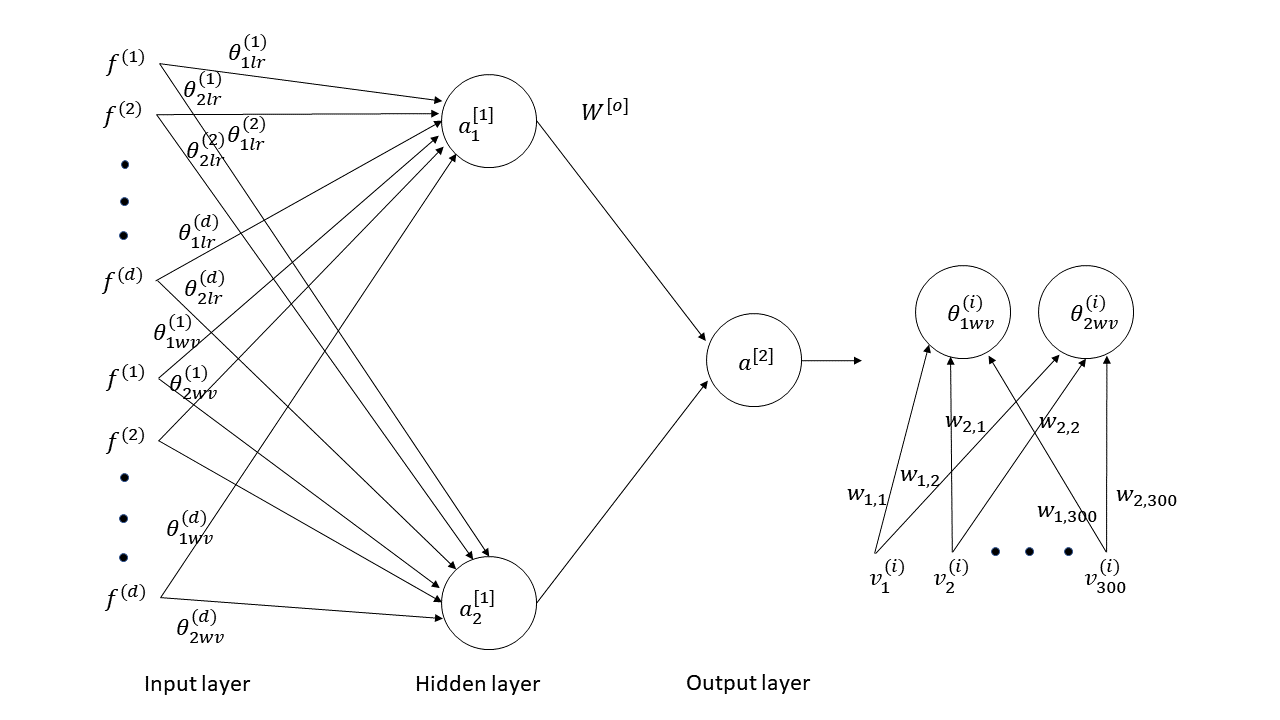
\includegraphics[width=16cm, height=10cm]{images/proposed_method_nn.png}\\
\centering
\caption{Neural network model - with word-vectors}
\label{fig:foo}
\end{figure}

Computing the weights through forward propagation and updating the weights through back propagation would be similar to the previous model.

\newpage
\subsection{Model Performance}

Below is a table showing how a neural network model with one hidden layer performed with and without using features generated by word-vectors.

\begin{table}[htbp]
\centering
\begin{tabular}{llllll}
\multicolumn{1}{l|}{Datasets}    & \multicolumn{1}{c|}{\begin{tabular}[c]{@{}c@{}}2 layer NN\\ Set Accuracy\end{tabular}} & \multicolumn{1}{c|}{\begin{tabular}[c]{@{}c@{}}2 layer NN with wv\\ Set Accuracy\end{tabular}} &  &  &  \\ \cline{1-3}
\multicolumn{1}{l|}{IMDb}        & \multicolumn{1}{c|}{18.21}                                                              & \multicolumn{1}{c|}{19.63}                                                                     &  &  &
\end{tabular}
\caption{\label{tab:widgets}Set-Accuracy Results}
\end{table}


\begin{table}[htbp]
\centering
\begin{tabular}{llllll}
\multicolumn{1}{l|}{Datasets}    & \multicolumn{1}{c|}{\begin{tabular}[c]{@{}c@{}}2 layer NN\\ Instance F1\end{tabular}} & \multicolumn{1}{c|}{\begin{tabular}[c]{@{}c@{}}2 layer NN with wv\\ Instance F1\end{tabular}} &  &  &  \\ \cline{1-3}
\multicolumn{1}{l|}{IMDb}        & \multicolumn{1}{c|}{56.14}                                                            & \multicolumn{1}{c|}{60.21}                                                                    &  &  &  \\
\multicolumn{1}{l|}{20NewsGroup} & \multicolumn{1}{c|}{55.64}                                                                 & \multicolumn{1}{c|}{58.97}                                                                    &  &  &  \\
\end{tabular}
\caption{\label{tab:widgets}Instance F1 Results}
\end{table}

We can see that for both the datasets, the neural network model using features generated by word-vectors is the better performing model. In fact this model even outperforms all other previously tested models.
